\chapter{Crossline Deblending (3D)} \label{chap:MahdadMethod3d}

This thesis suggests to blend crossline sources, i.e. in combination with the movement of the seismic vessel one effectively blends sources in 3D.

\todo[inline]{In this paragraph I use the word "source". For consistency I thought about using the word "shot". However, it seems to sound strange in this sentence.}

The deblending method of \citet{Mahdad-Deblending-Method} described in section \ref{sec:MahdadMethod} is designed for 2D blended data. In this thesis I will explain how each step of the Mahdad method can be applied to 3D data as well, and I will demonstrate its performance.

First, the data sorting will be modified such that the blended 3D data can be described using the same forward model as in section \ref{sec:Ch-Theory-Operator}. The presented data sorting will allow to maintain all other steps of the deblending algorithm of \citet{Mahdad-Deblending-Method} unchanged. Second, the $f$-$k$-filter will be extended to an $f$-$k_x$-$k_y$-filter to remove noise in crossline and inline direction.

\section{Data Sorting} \label{sec:Ch-Theory-3dExtension-DataSorting}

\subsection*{Data Matrix}

In 3D acquisition the sources and receivers are distributed on a 2D surface. Thus, their locations are defined by their crossline and inline positions, ($x$, $y$). Each data point which is measured by a source receiver pair at a specific time is therefore described by 5 coordinates, time $t$, receiver crossline and inline position ($x_r$, $y_r$), and source crossline and inline position ($x_s$, $y_s$).

The 5D data "cube" will be again reorganized in a 2D data matrix according to \citet{Delphi-Format} (see Figure \ref{fig:Ch-Theory-DelphiFormat}). For this data sorting a 1D Fourier transform with respect to time is performed and a 4D frequency "slice" is selected.

The 4D "slice" is sorted in a 2D data matrix, $\mathbf{P}$, with as many rows as receivers and as many columns as shots. The total number of shots is obtained by multiplying the number of shots fired in each crossline and the number of shots fired in each inline. The total number of receivers is obtained likewise. Assume there are $Ns_x$ shots per crossline. The shots of the first crossline are assigned to the first $Ns_x$ columns of the data matrix, the shots of the second crossline are assigned to the next $Ns_x$ columns of the data matrix, etc. The cross- and inline receivers are sorted in the rows of the data matrix in analogy.

For example, one row in the data matrix, $\mathbf{P}$, in Figure \ref{fig:Ch-Theory-DelphiFormat} represents  a common receiver gather. The data of this common receiver gather are shown in Figure \ref{fig:Ch-Theory-Data3d}, where the coordinates, $x$ and $y$, indicate the crossline and inline shot position respectively. For the described data sorting individual crossline slices are extracted from this data cube and assembled next to each other in a data matrix as shown in Figure \ref{fig:Ch-Theory-Data3d_Delphi}. Each hyperbolic event refers to the response of the shots of one crossline.

\begin{figure}
	\centering
	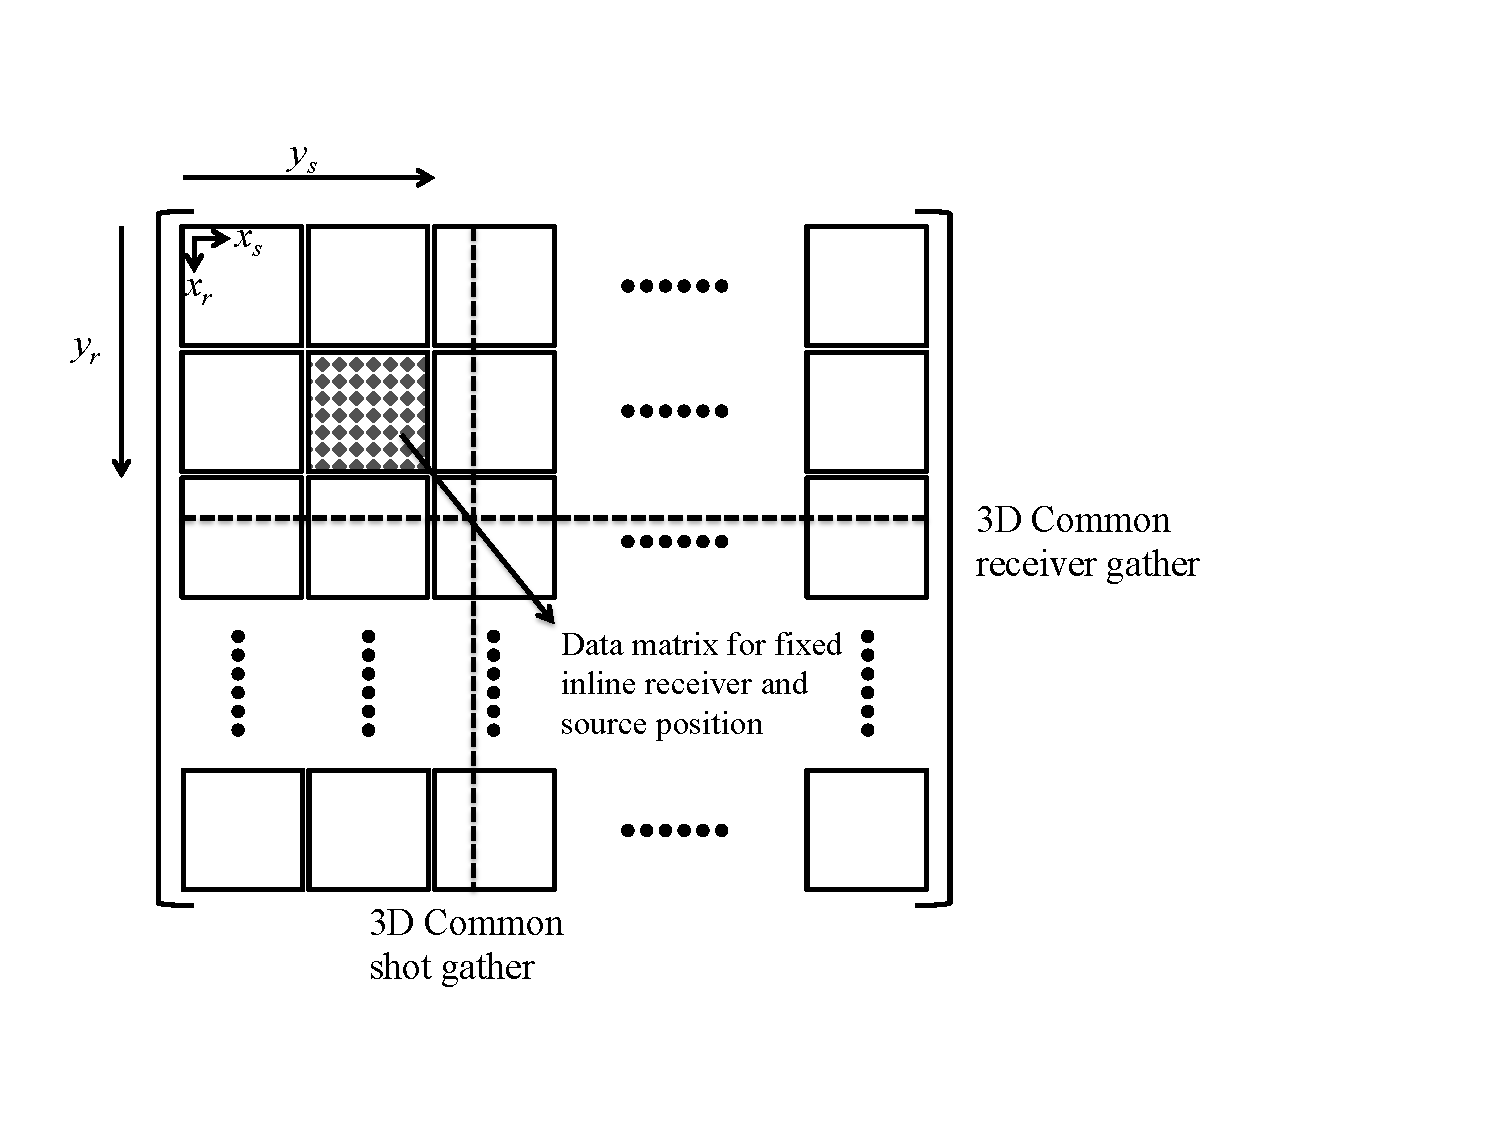
\includegraphics[width=0.6\textwidth]{Plots/DelphiFormat-v2}
	\caption{Illustration of the data matrix $\mathbf{P}$ for 3D data \citep{Delphi-Format}. $y_r$ and $y_s$ represent the inline receiver and source positions. $x_r$ and $x_s$ represent the crossline receiver and source positions. Each row refers to a 3D common receiver gather and each column to a 3D common shot gather. A sub-matrix with fixed receiver and source inline positions ($y_r$, $y_s$) is equivalent to a data matrix for 2D acquisition.}
	\label{fig:Ch-Theory-DelphiFormat}
\end{figure}


\begin{figure}
	
	\begin{subfigure}[t]{\textwidth}
	 	\centering
		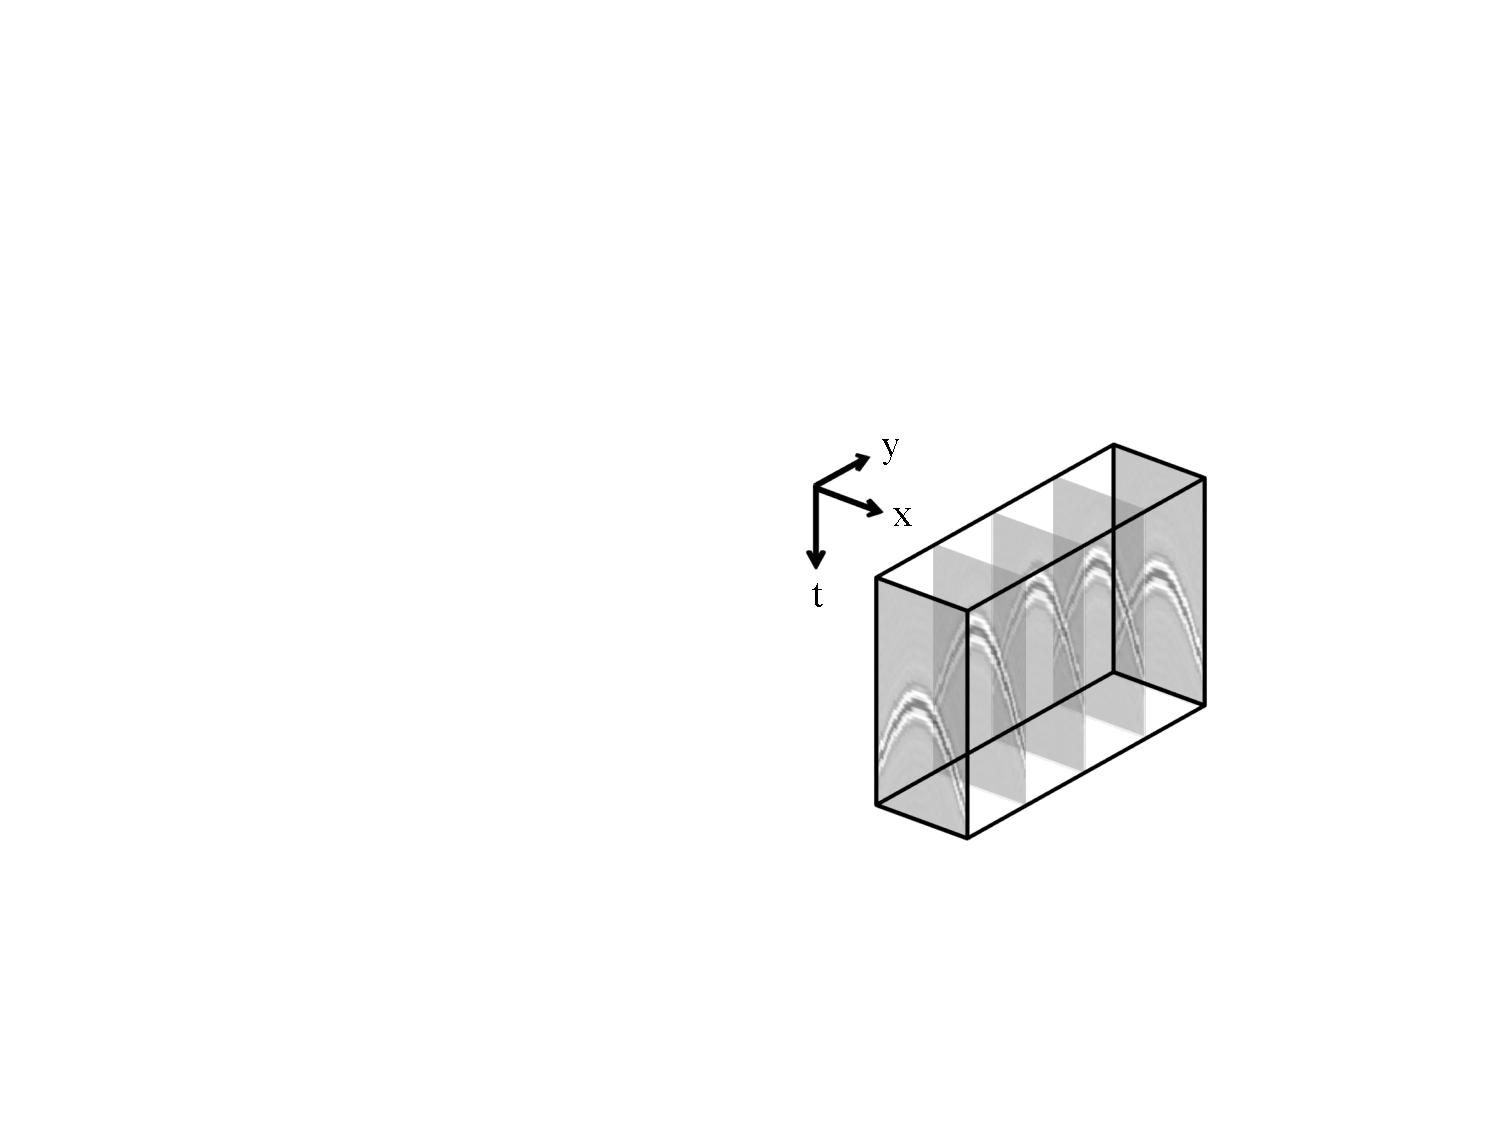
\includegraphics[width = 0.3\textwidth]{Plots/data3d}
		\caption{}
		\label{fig:Ch-Theory-Data3d}
	\end{subfigure}
	\par\bigskip
	\begin{subfigure}[t]{\textwidth}
		\centering
		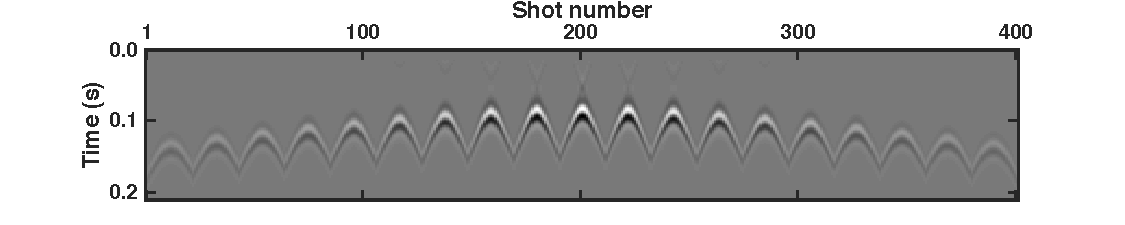
\includegraphics[width = \textwidth]{Plots/IdealData3d/p_Delphi}
		\caption{}
		\label{fig:Ch-Theory-Data3d_Delphi}
	\end{subfigure}
	
	\caption{(a) Common receiver gather of a 3D data set with crossline (x) and inline (y) sources. (b) Resorted data set. Individual crossline sections are plotted next to each other in 2D. For visibility both subfigures only show a reduced part of the data.}
	\label{fig:Ch-Theory-DataSorting}
\end{figure}


\subsection*{Blending matrix}

The blending matrix for 3D is build in a similar fashion as the data matrix in 3D. As described in section \ref{sec:BlendingMatrix} each row of the blending matrix, $\mathbf{\Gamma}$, captures one shot. For extension to 3D the shots of the first crossline are placed in the top $Ns_x$ rows of the blending matrix, followed by the shots of the second crossline etc. (see Figure \ref{fig:Ch-Theory-3D-BlendingMatrix-Design}). The elements in the $j^{th}$ column of the blending matrix, $\mathbf{\Gamma}$, select the shots which are blended in the $j^{th}$ experiment. For example, the first column of the blending matrix in Figure \ref{fig:Ch-Theory-3D-BlendingMatrix} describes that in the first experiment shots $1$ and $3$ are blended with a time delay of $\Delta t_1$.

\todo[inline]{Keep this sentence for later: This framework allows to blend any source combination independent of the cross- and inline positions of the involved sources.}

With the new data and blending matrix sorting one can apply deblending to 3D data.

\begin{figure}

	\begin{subfigure}[t]{0.5\textwidth}
		\centering
		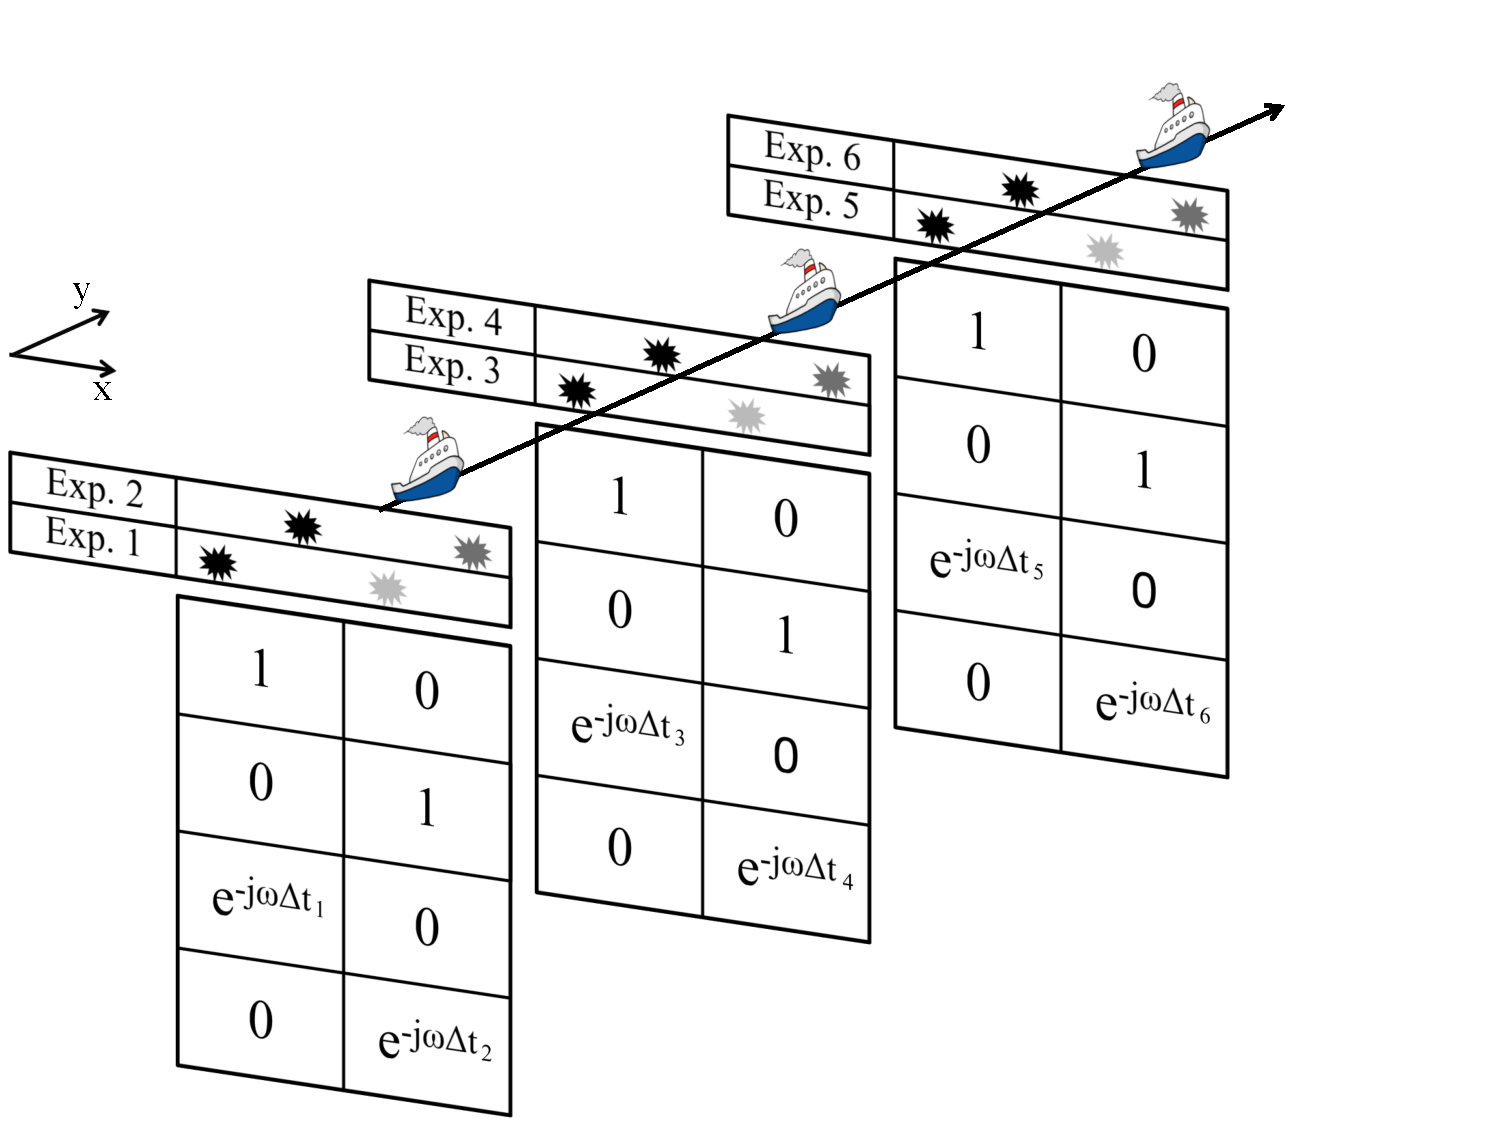
\includegraphics[width = \textwidth]{Plots/DrawingsCartesianFormat1}
		\caption{}
		\label{fig:Ch-Theory-3D-BlendedAcquisition}
	\end{subfigure}
	%
	\begin{subfigure}[t]{0.5\textwidth}
		\centering
		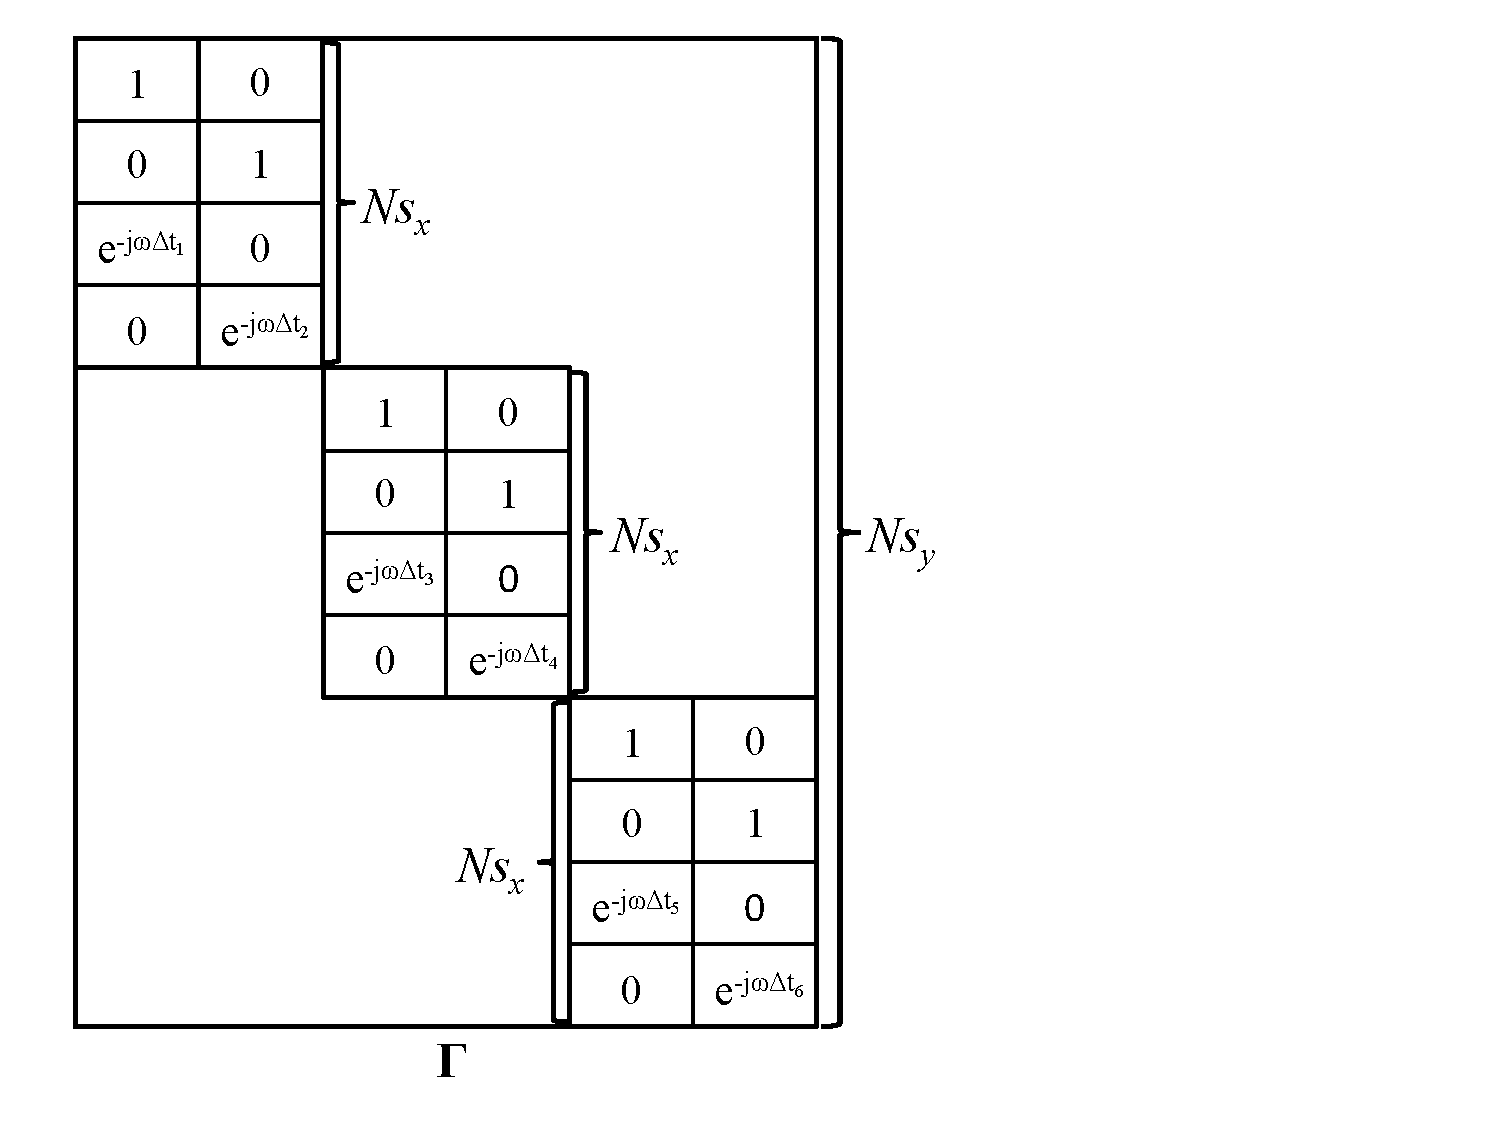
\includegraphics[width = 0.7\textwidth]{Plots/DrawingsCartesianFormat2}
		\caption{}
		\label{fig:Ch-Theory-3D-BlendingMatrix}
	\end{subfigure}
	
	\caption{Illustration of the blending matrix, $\mathbf{\Gamma}$, for 3D acquisition. (a) At each of the $Ns_y$ inline position the crossline sources ($x$ direction) are blended. Each of these 2D blending processes is described by a 2D blending matrix, which has as many rows as there are crossline sources, $Ns_x$. (b) The 2D blending matrices are assembled in a single 3D blending matrix, $\mathbf{\Gamma}$, which has $Ns_x$ by $Ns_y$ rows.}
	\label{fig:Ch-Theory-3D-BlendingMatrix-Design}

\end{figure}


\section{3D f-k-k Filter} \label{sec:Ch-Theory-3dExtension-FKK}

In section \ref{sec:IterBlenNoiseEst} the 2D $f$-$k$ filter was introduced. By sorting the 2D $f$-$k$-fitler according to section \ref{sec:Ch-Theory-3dExtension-DataSorting} it can be applied to 3D data. 

For this purpose one considers a 3D common receiver gather, $\mathbf{p}(t,x_s,y_s)$, and brings it to the $f$-$k_x$-$k_y$ domain by applying a 3-dimensional Fourier transform. Next, a constant frequency slice is selected. This leaves a 2D matrix, which captures the cross- and inline wavenumbers ($k_x$, $k_y$). The maximum crossline wavenumber, $k_x$, is defined according to section \ref{sec:IterBlenNoiseEst}. The resulting $f$-$k$-mask is shown in Figure \ref{fig:Ch-Mahdad3d-2dfk}. Note that it only filters the crossline wavenumbers $k_x$, i.e. it is a $f$-$k_x$ filter.

The $f$-$k_x$-$k_y$ spectra of synthetic data shown in Figure \ref{fig:Ch-Theory-FK-f_slice-data} and \ref{fig:Ch-Theory-FK-delphi-data} illustrate that the 2D $f$-$k_x$-filter will also pass some energy which is not signal. In the following both spatial directions, $x$ and $y$, are considered to extend the filter to a 3D $f$-$k_x$-$k_y$-filter.

\begin{figure}

	\centering 
	\begin{subfigure}[t]{0.45\textwidth}
		\centering
		\includegraphics[width = 0.65\textwidth]{Plots/IdealData3d/fkk-mask-slice40-2d}
		\caption{}
		\label{fig:Ch-Mahdad3d-2dfk-slice}
	\end{subfigure}
	
	\par\bigskip
	
	\centering
	\begin{subfigure}[t]{\textwidth}
		\centering
		\includegraphics[width = 0.9\textwidth]{Plots/IdealData3d/fkk-mask-Delphi-2d}
		\caption{}
		\label{fig:Ch-Mahdad3d-2dfk-Delphi}
	\end{subfigure}
	
	\caption{One can design a 2D $f$-$k_x$-filter for 3D data. (a) shows a \SI{40}{\hertz} frequency slice of the $f$-$k_x$-$k_y$ spectrum, where the shite area equals 1 and the black area is 0. Note that the filter is not affecting the inline wavenumbers $k_y$. (b) illustrates the 2D $f$-$k_x$-filter sorted according to section \ref{sec:Ch-Theory-3dExtension-DataSorting}. Each cone represents a 2D $f$-$k$-filter for a single inline wavenumber.}
	\label{fig:Ch-Mahdad3d-2dfk}
\end{figure}

The starting point is a frequency slice of the $f$-$k_x$-$ky$ spectrum as shown in Figure \ref{fig:Ch-Theory-FK-f_slice-data}. Again the minimum velocity, $v_{min}$, and the frequency, $f$, determine the maximum wavenumber, $k_{max}$, according to equation \ref{eq_Ch-Theory-MaxWavenmber}. The total wavenumber, $k_{T}$, must be smaller than the maximum wavenumber, $k_{max}$,

\begin{equation}
	k_{T} = \sqrt{k_x^2 + k_{y}^2} < k_{max}.
	\label{eq:Ch-Theory-TotalWavenumber}
\end{equation}

Hence the signal "cone" is defined by a circle (see Figure \ref{fig:Ch-Theory-FK-f_slice-mask}). This is repeated for each frequency component, such that the overall $f$-$k_x$-$k_y$-mask is a 3D cone (see Figure \ref{fig:Ch-Theory-FKK-Mask}). Finally, this mask is computed for each receiver gather.

\begin{comment}
Once the mask is built for a 5D data array it can either be applied to filter a 5D data array, or the mask is sorted to 2D according to section \ref{sec:Ch-Theory-3dExtension-DataSorting}, and applied to the $f$-$k_x$-$k_y$-spectrum of the data matrix (see Figure \ref{fig:Ch-Theory-FK-delphi-data}, \ref{fig:Ch-Theory-FK-delphi-mask}).
\end{comment}

\begin{figure}
	\centering
	\begin{subfigure}[t]{0.3\textwidth}
		\centering
		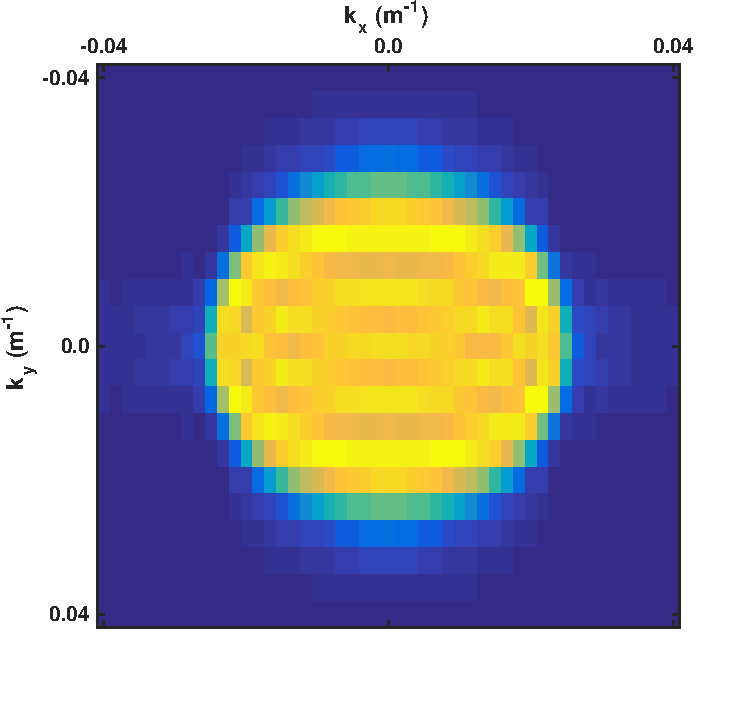
\includegraphics[width=\textwidth]{Plots/IdealData3d/P_f_slice40}
		\caption{}
		\label{fig:Ch-Theory-FK-f_slice-data}
	\end{subfigure}
	%
	\centering
	\begin{subfigure}[t]{0.3\textwidth}
		\centering
		\includegraphics[width=\textwidth]{Plots/IdealData3d/fk-slices/3dfk-cone}
		\caption{}
		\label{fig:Ch-Theory-FK-f_slice-data3d}
	\end{subfigure}
	%
	\centering
	\begin{subfigure}[t]{0.3\textwidth}
		\centering
		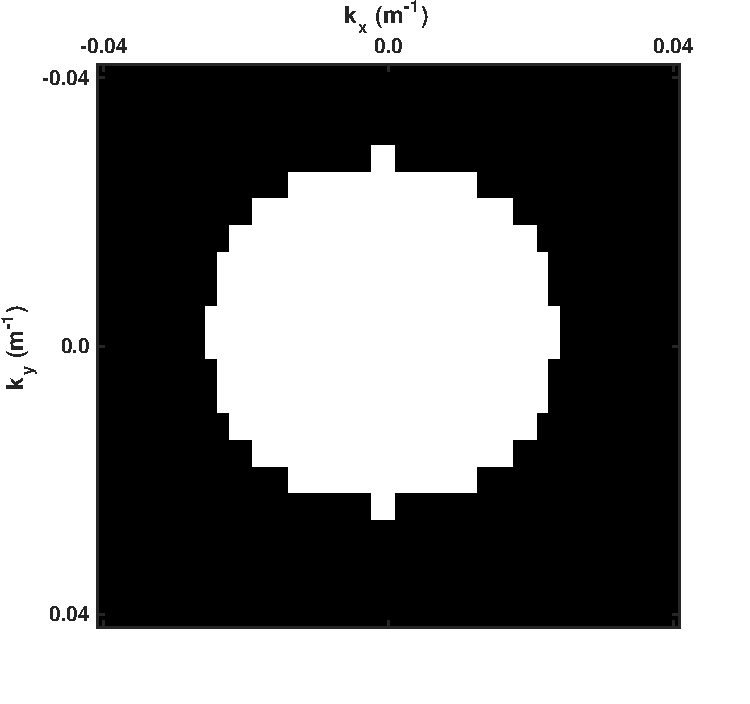
\includegraphics[width=\textwidth]{Plots/IdealData3d/fkk-mask-slice40}
		\caption{}
		\label{fig:Ch-Theory-FK-f_slice-mask}
	\end{subfigure}
	
	\begin{subfigure}[t]{\textwidth}
		\centering
		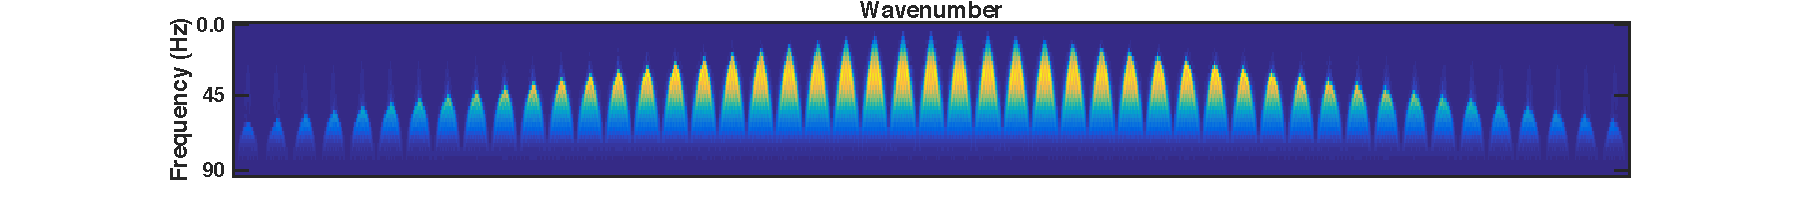
\includegraphics[width=0.9\textwidth]{Plots/IdealData3d/P_fkk_Delphi}
		\caption{}
		\label{fig:Ch-Theory-FK-delphi-data}
	\end{subfigure}
	\par\bigskip
	\begin{subfigure}[t]{\textwidth}
		\centering
		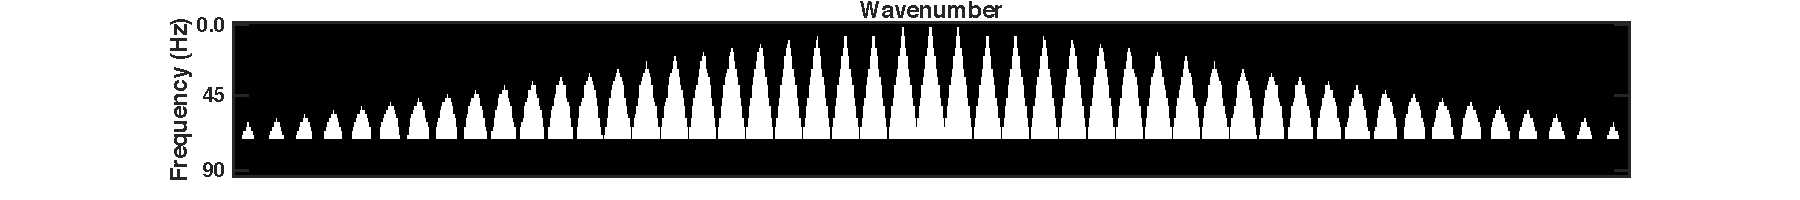
\includegraphics[width=0.9\textwidth]{Plots/IdealData3d/fkk-mask-Delphi}
		\caption{}
		\label{fig:Ch-Theory-FK-delphi-mask}
	\end{subfigure}
	
	\caption{Illustration of the 3D $f$-$k_x$-$k_y$-filter. (a) is a \SI{40}{\hertz} frequency slice of the $f$-$k_x$-$k_y$ spectrum of the data in Figure \ref{fig:Ch-Theory-Data3d_Delphi}. $k_x$ and $k_y$ refer to the crossline and inline wavenumber respectively. (b) shows the same data slice sorted in a 3D cube. The red cone represents the 3D $f$-$k_x$-$k_y$ filter mask. (c) is a \SI{40}{\hertz} frequency slice of the mask, where the white area equals 1 and the black area is 0. (d) and (e) display the $f$-$k_x$-$k_y$ data spectrum and mask sorted according to section \ref{sec:Ch-Theory-3dExtension-DataSorting}, i.e. each sub-cone refers to one inline wavenumber. Note that due to the sorting the wavenumber axis is a mix of crossline and inline wavenumbers. For this reason the wavenumber axis has no labels.}
	\label{fig:Ch-Theory-FKK-Mask}

\end{figure}



\section{Results}

The 3D $f$-$k_x$-$k_y$ filter removes incoherent energy in the crossline and inline direction. The suggested 3D blended acquisition design blends sources within the same crossline. Hence, the question arouses whether an extension of the 2D $f$-$k_x$ filter to the inline direction provides significant deblending enhancements.

For this purpose the synthetic data of Figure \ref{fig:Ch-Mahdad3d-Unbl-Delphi} are blended: Within each crossline there are 21 sources, which are blended in 3 experiments. For each experiment 7 randomly selected sources are blended with random time delays, i.e. the blending pattern with mixed incoherency is applied. The maximum allowed firing time delay is set to \SI{400}{\milli\second}. 

The blended data are deblended with the 3D deblending algorithm. In one case a 2D $f$-$k_x$ filter is applied (see Figure \ref{fig:Ch-Mahdad3d-Deblending-2dfk}). In the other case a 3D $f$-$k_x$-$k_y$ filter is applied (see Figure \ref{fig:Ch-Mahdad3d-Deblending-3dfk}). It is clearly visible that the deblending quality increases significantly with the 3D $f$-$k_x$-$k_y$ filter.

In order to quantify the quality gap between the results with 2D and 3D filters, the data of Figure \ref{fig:Ch-Mahdad3d-Unbl-Delphi} are blended with maximum firing time delays varying between \SI{40}{\milli\second} and \SI{400}{\milli\second}. The blended data are deblended in one case with a 2D $f$-$k$ filter, and in the other case with a 3D $f$-$k_x$-$k_y$ filter. The resulting quality factors are shown in Figure \ref{fig:Ch-Mahdad3d-2dvs3dfk}.

 
\begin{figure}
	
	\centering
	\begin{subfigure}[t]{0.8\textwidth}
		\centering
		\includegraphics[width = \textwidth]{Plots/BlendingPatterns/Unblended_Delphi_zoom-font14}
		\caption{Unblended synthetic data. These data show a common receiver gather, which is generated by 21 crossline shots and 51 inline shots. The shown section is a zoom on the strongest events.}
		\label{fig:Ch-Mahdad3d-Unbl-Delphi}
	\end{subfigure}

	\par\bigskip

	\centering
	\begin{subfigure}[t]{0.8\textwidth}
		\includegraphics[width = \textwidth]{Plots/2dvs3dfk/Deblendedv6_xt_100}
		\caption{Deblending result with a 2D $f$-$k_x$ filter}
		\label{fig:Ch-Mahdad3d-Deblending-2dfk}
	\end{subfigure}
	
	\par\bigskip
	
	\centering
	\begin{subfigure}[t]{0.8\textwidth}
		\includegraphics[width = \textwidth]{Plots/2dvs3dfk/Deblendedv5_xt_100}
		\caption{Deblending result with a 3D $f$-$k_x$-$k_y$ filter}
		\label{fig:Ch-Mahdad3d-Deblending-3dfk}
	\end{subfigure}
	
	\caption{The crossline sources of the synthetic data in Figure \ref{fig:Ch-Results-Unbl-Delphi} are blended. Then, the 3D deblending algorithm is applied. In case (a) the algorithm uses a 2D $f$-$k_x$ filter. In case (b) it uses a 3D $f$-$k_x$-$k_y$ filter.}
	\label{fig:Ch-Mahdad3d-Deblending-2dvs3d-fk}
	
\end{figure}



\begin{figure}
	\centering
	\includegraphics[width = 0.6\textwidth]{Plots/2dvs3dfk/Q_2d-vs-3d_fk}
	\caption{Comparison of the deblending quality with a 2D $f$-$k_x$ filter and a 3D $f$-$k_x$-$k_y$ filter. The data in Figure \ref{fig:Ch-Mahdad3d-Unbl-Delphi} are blended with varying maximum firing time delay. Then the blended data are deblended using a 2D $f$-$k_x$ filter and a 3D $f$-$k_x$-$k_y$ filter.}
	\label{fig:Ch-Mahdad3d-2dvs3dfk}
\end{figure}


















